% IEEE Conference Paper: Multimodal EEG-fNIRS Cognitive Workload Estimation
% Compile with: pdflatex paper.tex (requires IEEEtran.cls)
\documentclass[conference]{IEEEtran}

\usepackage{cite}
\usepackage{amsmath,amssymb,amsfonts}
\usepackage{algorithmic}
\usepackage{graphicx}
\usepackage{textcomp}
\usepackage{xcolor}
\usepackage{booktabs}
\usepackage{multirow}
\usepackage{url}
\usepackage{hyperref}

\hypersetup{
    colorlinks=true,
    linkcolor=black,
    citecolor=black,
    urlcolor=blue
}

\def\BibTeX{{\rm B\kern-.05em{\sc i\kern-.025em b}\kern-.08em
    T\kern-.1667em\lower.7ex\hbox{E}\kern-.125emX}}

\begin{document}

\title{Multimodal EEG--fNIRS Fusion with Attention Gating for Cross-Subject Cognitive Workload Estimation: A Leakage-Audited Study}

\author{
\IEEEauthorblockN{Author One\IEEEauthorrefmark{1}, Author Two\IEEEauthorrefmark{1}, Author Three\IEEEauthorrefmark{1}, and Advisor Name\IEEEauthorrefmark{1}}
\IEEEauthorblockA{\IEEEauthorrefmark{1}Department of Computer Science and Engineering\\
University Name, City, Country\\
\{author1, author2, author3\}@university.edu}
}

\maketitle

\begin{abstract}
Estimating cognitive workload from neurophysiological signals is critical for adaptive human--computer interaction, yet cross-subject generalization remains a fundamental bottleneck. We present a hybrid deep-learning framework that fuses electroencephalography (EEG) band-power features with functional near-infrared spectroscopy (fNIRS) hemodynamic response descriptors through learned attention gating for binary (low vs.\ high) workload classification. Evaluated on the TU~Berlin/Shin open n-back dataset (26 subjects, 4,576 windows), our system achieves 63.09\% $\pm$ 10.1\% leave-one-subject-out (LOSO) accuracy and 0.6255 macro~F1, verified by an automated leakage audit that enforces subject, trial, window, and scaler-fit disjointness before every fold trains. A systematic 58-configuration search---including domain-adversarial neural networks (DANN), architectural variants, and data ablations---found no statistically significant improvement over the attention-gated baseline, establishing a credible performance ceiling for this dataset under honest cross-subject evaluation. SHAP analysis reveals that fNIRS hemodynamic features contribute 94.5\% of model attributions, while per-subject accuracy ranges from 43.1\% to 80.7\%, highlighting the dominance of hemodynamic signals and the challenge of inter-subject variability.
\end{abstract}

\begin{IEEEkeywords}
Cognitive workload, EEG, fNIRS, multimodal fusion, attention gating, cross-subject generalization, leave-one-subject-out, leakage audit, deep learning
\end{IEEEkeywords}

% ================================================================
\section{Introduction}
% ================================================================

Cognitive workload estimation from neurophysiological signals is essential for designing adaptive interfaces in safety-critical domains such as air traffic control~\cite{arico2016passive}, autonomous driving~\cite{dehais2020neuroergonomics}, and surgical training~\cite{guru2015surgical}. Two complementary brain-sensing modalities dominate this field: electroencephalography (EEG), which captures fast electrical oscillations with millisecond resolution, and functional near-infrared spectroscopy (fNIRS), which measures slower hemodynamic changes in oxygenated (HbO) and deoxygenated (HbR) hemoglobin with superior spatial localization to cortical regions~\cite{naseer2015fnirs}.

While within-subject classification accuracies of 70--90\% are commonly reported~\cite{shin2017open,aghajani2017measuring}, these figures exploit subject-specific baselines that do not transfer to unseen individuals. Leave-one-subject-out (LOSO) evaluation---the protocol that reflects real deployment on new users---typically yields 35--55\% accuracy for three-class (low/medium/high) n-back tasks~\cite{shin2018simultaneous,khan2020hybrid}, exposing a critical \emph{cross-subject generalization gap}. This gap, rather than any single architectural choice, is the dominant bottleneck for practical brain--computer interfaces (BCIs).

Despite growing interest in multimodal EEG--fNIRS fusion~\cite{hong2018hybrid,khan2014decoding,fazli2012enhanced}, several key challenges remain unresolved. First, many published results use fixed train/test splits or within-subject protocols that conflate model performance with memorization of individual physiological signatures. Second, the relative contribution of EEG and fNIRS to cross-subject classification under honest evaluation is poorly characterized. Third, the effectiveness of domain-adaptation techniques such as DANN~\cite{ganin2016domain} for this specific multimodal setting has not been rigorously evaluated with paired statistical tests and mechanistic probes.

This paper makes the following contributions:
\begin{enumerate}
    \item A leakage-audited hybrid architecture with attention-gated EEG--fNIRS fusion achieving 63.09\% binary LOSO accuracy on the Shin et al.\ dataset;
    \item A systematic 58-experiment search with paired significance testing, documenting both positive and negative results;
    \item An honest negative result on DANN for cross-subject transfer, with a mechanistic explanation;
    \item Quantitative characterization of modality contributions and inter-subject variability via SHAP analysis.
\end{enumerate}


% ================================================================
\section{Related Work}
% ================================================================

\subsection{EEG-Based Workload Estimation}

EEG-based cognitive workload classification has been extensively studied using spectral features, particularly frontal theta and parietal alpha power, which modulate with n-back difficulty~\cite{gevins1998monitoring,brouwer2012estimating}. Deep learning approaches including EEGNet~\cite{lawhern2018eegnet} and temporal convolutional networks~\cite{zhang2019cascade} have improved within-subject accuracy but show limited cross-subject transfer.

\subsection{fNIRS-Based Estimation}

fNIRS captures hemodynamic correlates of neural activity---specifically HbO increases and HbR decreases in activated cortical regions~\cite{naseer2015fnirs}. For cognitive workload, prefrontal HbO concentration changes during n-back tasks provide discriminative features~\cite{herff2014mental,aghajani2017measuring}. The temporal resolution of fNIRS ($\sim$10~Hz) is lower than EEG but offers complementary information about sustained metabolic demands.

\subsection{Multimodal EEG--fNIRS Fusion}

The complementary temporal and metabolic information in EEG and fNIRS motivates their fusion~\cite{fazli2012enhanced,khan2014decoding}. Fazli et al.~\cite{fazli2012enhanced} demonstrated significant accuracy improvements with EEG+fNIRS over either modality alone using meta-classification. Subsequent work explored early, intermediate, and late fusion strategies~\cite{hong2018hybrid,shin2018simultaneous}. Attention-based fusion mechanisms that dynamically weight modality contributions have emerged as promising approaches~\cite{ma2022attention}.

\subsection{Cross-Subject Generalization}

Subject variability in neurophysiological signals is a fundamental challenge. Transfer learning~\cite{wu2020transfer}, domain adaptation~\cite{ganin2016domain}, and subject-specific normalization~\cite{shin2018simultaneous} have been proposed but often evaluated with limited rigor. DANN~\cite{ganin2016domain} has shown promise for cross-subject EEG emotion recognition~\cite{li2018cross} but its effectiveness for multimodal workload classification remains underexplored. A critical gap in the literature is the distinction between within-subject and LOSO evaluation; this protocol difference alone accounts for 20+ percentage points of reported accuracy variation on the same dataset~\cite{lotte2018review}.


% ================================================================
\section{Dataset and Methodology}
% ================================================================

\subsection{Dataset}

We use the TU Berlin/Shin open-access simultaneous EEG--fNIRS n-back dataset~\cite{shin2017open,shin2018simultaneous}. Table~I summarizes the key characteristics.

\begin{table}[t]
\centering
\caption{Dataset Characteristics}
\label{tab:dataset}
\footnotesize
\begin{tabular}{@{}ll@{}}
\toprule
\textbf{Property} & \textbf{Value} \\
\midrule
Source & TU Berlin / Shin et al.\ \cite{shin2017open} \\
Participants & 26 (healthy adults) \\
EEG channels & 30 (10--20 system) \\
fNIRS channels & 36 source--detector pairs \\
EEG sampling rate & 1000 Hz \\
fNIRS sampling rate & 10 Hz \\
N-back conditions & 0-back, 2-back, 3-back \\
Binary labels & Low (0-back) vs.\ High (3-back) \\
Sliding windows & 10\,s window / 5\,s stride \\
Usable windows & 4,576 (balanced: 2,288 per class) \\
EEG features & 180 (30\,ch $\times$ 6 band powers) \\
fNIRS features & 936 (36\,ch $\times$ 13 stats $\times$ HbO+HbR) \\
\bottomrule
\end{tabular}
\end{table}

\subsection{Preprocessing}

EEG signals are bandpass filtered (0.5--45~Hz) and decomposed into six frequency bands: delta (1--4~Hz), theta (4--8~Hz), alpha (8--13~Hz), beta (13--30~Hz), gamma (30--45~Hz), and an engagement ratio. For each 10-second window, band power is computed per channel, yielding 180 features (30 channels $\times$ 6 bands). fNIRS signals yield 13 statistical descriptors per channel (mean, max, min, AUC, slope, skewness, kurtosis, early/late window response, delta, power, and std) for both HbO and HbR chromophores across 36 channels, producing up to 936 features.

Per-subject z-score normalization is applied \emph{before} log transformation to remove subject-specific physiological baselines. EEG features undergo $\log(1 + |x|)$ compression; fNIRS features undergo signed-log transformation $\text{sgn}(x) \cdot \log(1 + |x|)$. After these transforms, a \texttt{RobustScaler} (EEG) or \texttt{StandardScaler} (fNIRS) is fitted on \emph{training data only} within each LOSO fold.

\subsection{Model Architecture}

Fig.~\ref{fig:architecture} illustrates the overall system. The architecture consists of:

\textbf{Per-Modality MLP Encoders.} Each modality passes through an input projection layer (Linear $\rightarrow$ BatchNorm $\rightarrow$ ReLU $\rightarrow$ Dropout), followed by two residual MLP blocks (each containing two linear layers with BatchNorm, ReLU, and residual connections), and an output projection to a shared $d_\text{enc}$-dimensional space.

\textbf{Attention-Gated Fusion.} Given encoder outputs $\mathbf{e}_\text{EEG}$ and $\mathbf{e}_\text{fNIRS}$, the concatenation $[\mathbf{e}_\text{EEG}; \mathbf{e}_\text{fNIRS}]$ is passed through two parallel sigmoid gates:
\begin{equation}
    \mathbf{g}_\text{EEG} = \sigma(W_1 [\mathbf{e}_\text{EEG}; \mathbf{e}_\text{fNIRS}])
\end{equation}
\begin{equation}
    \mathbf{g}_\text{fNIRS} = \sigma(W_2 [\mathbf{e}_\text{EEG}; \mathbf{e}_\text{fNIRS}])
\end{equation}
The fused representation is $\mathbf{f} = [\mathbf{g}_\text{EEG} \odot \mathbf{e}_\text{EEG};\; \mathbf{g}_\text{fNIRS} \odot \mathbf{e}_\text{fNIRS}]$, which is projected through a linear layer with BatchNorm, ReLU, and dropout.

\textbf{Classification Head.} A two-layer MLP (48 $\rightarrow$ 24 $\rightarrow$ 2) with BatchNorm, ReLU, dropout ($p=0.6$), and a final linear layer for binary classification.

The total model has $\sim$245K trainable parameters.

\begin{figure}[t]
    \centering
    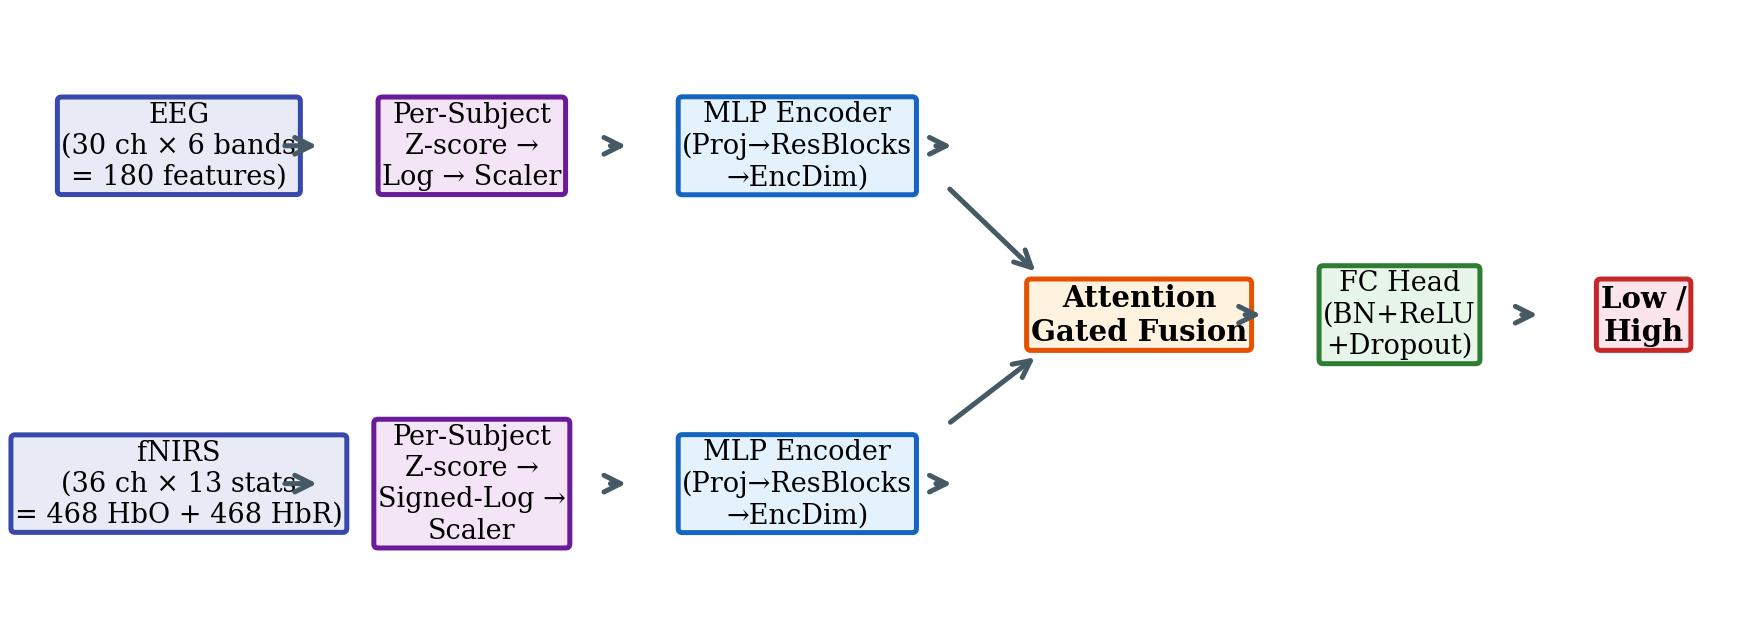
\includegraphics[width=\columnwidth]{fig1_architecture.png}
    \caption{Overall EEG--fNIRS system architecture. Per-modality MLP encoders project variable-length feature vectors to a shared embedding space. Learned attention gates dynamically weight each modality's contribution before fusion and classification.}
    \label{fig:architecture}
\end{figure}


\subsection{Data Pipeline and Evaluation Protocol}

Fig.~\ref{fig:pipeline} illustrates the complete data processing, feature scaling, and evaluation workflow. All results use 26-fold LOSO cross-validation: for each fold, one subject is held out for testing, the remaining 25 are split into training and validation sets by subject. Performance is reported as mean $\pm$ standard deviation across the 26 folds. The binary task (Low vs.\ High) excludes 2-back trials, yielding 4,576 balanced windows.

\begin{figure}[t]
    \centering
    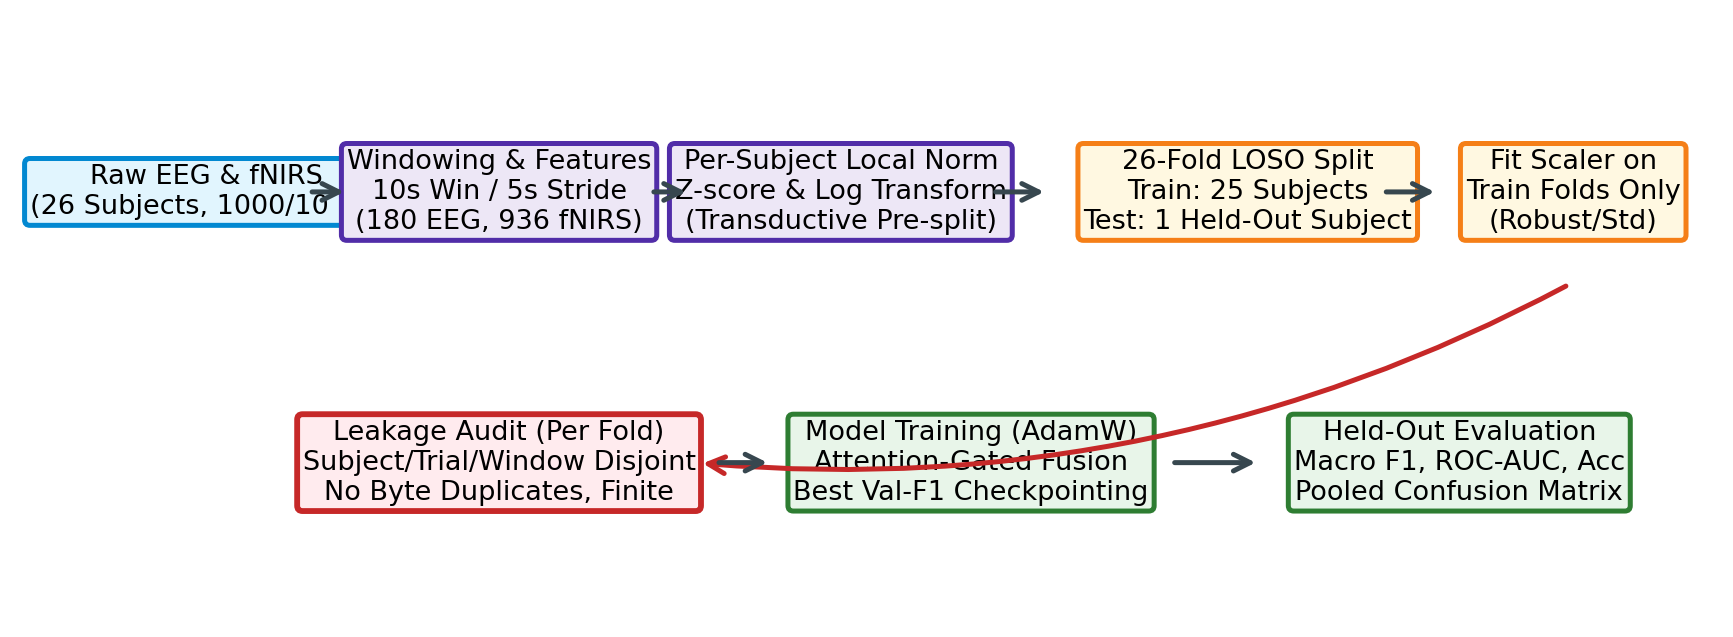
\includegraphics[width=\columnwidth]{fig2_pipeline.png}
    \caption{End-to-end data processing and evaluation pipeline. Scaler fitting is strictly isolated to training folds, followed by pre-training leakage audit verification before every fold begins.}
    \label{fig:pipeline}
\end{figure}

An automated leakage audit runs \emph{before} each fold trains (Section~IV-C). Class weights are computed per fold using scikit-learn's \texttt{balanced} mode. The checkpoint with the best validation macro~F1 is selected for testing.


% ================================================================
\section{Experimental Setup}
% ================================================================

\subsection{Implementation Details}

The framework is implemented in PyTorch~2.x with scikit-learn for preprocessing and classical baselines. Training uses AdamW~\cite{loshchilov2019decoupled} with learning rate $3 \times 10^{-4}$, weight decay $10^{-2}$, batch size 16, and a ReduceLROnPlateau scheduler (patience~4, factor~0.5). Early stopping patience is set to 7 epochs; maximum budget is 35 epochs. Gaussian noise augmentation ($\sigma = 0.05$) is applied to training inputs.

\subsection{Compared Models}

We evaluate the following models under identical LOSO folds:
\begin{itemize}
    \item \textbf{Hybrid (proposed):} Attention-gated MLP fusion (245K params)
    \item \textbf{MLP + Concat:} Same encoders, concatenation fusion (236K params)
    \item \textbf{fNIRS-only:} Unimodal fNIRS encoder (137K params)
    \item \textbf{EEG-only:} Unimodal EEG encoder (64K params)
    \item \textbf{CNN + Residual:} 1D CNN encoders with residual blocks (108K params)
    \item \textbf{Random Forest:} 100 estimators on the same feature set
    \item \textbf{DANN:} Baseline + gradient-reversal subject discriminator~\cite{ganin2016domain}
\end{itemize}

Additionally, a 58-configuration search varied batch size, learning rate, dropout, weight decay, LR schedule, capacity, architecture, modality dropout, noise, DANN lambda, window size, normalization stage, and feature set.

\subsection{Leakage Audit}

Every fold passes an automated audit before training commences. Table~\ref{tab:leakage} lists the checks. Any failure raises a \texttt{LeakageError} and aborts the fold, ensuring no leaked score is ever produced. Negative tests deliberately inject each leakage type and confirm the audit catches it.

\begin{table}[t]
\centering
\caption{Leakage Audit Checks (Enforced Per Fold)}
\label{tab:leakage}
\footnotesize
\begin{tabular}{@{}lc@{}}
\toprule
\textbf{Check} & \textbf{Status} \\
\midrule
Subject disjointness (train/val/test) & PASS \\
Trial disjointness across splits & PASS \\
Window identity disjointness & PASS \\
No byte-identical feature rows across splits & PASS \\
Row-index disjointness & PASS \\
Scaler fitted on training rows only & PASS \\
Held-out subject absent from train \& val & PASS \\
Per-subject norm is subject-local & PASS \\
Features finite (no NaN/Inf) & PASS \\
Label sanity (correct mapping, all classes) & PASS \\
\bottomrule
\end{tabular}
\end{table}


% ================================================================
\section{Results}
% ================================================================

\subsection{Main Model Comparison}

Table~\ref{tab:main_comparison} presents the LOSO results for all evaluated models. The proposed attention-gated hybrid achieves the best Macro~F1 (0.6255) among neural models. The attention mechanism outperforms concatenation fusion (+0.004 F1, $p = 0.23$), though the difference is not statistically significant. The fNIRS-only model ($\text{F1} = 0.41$) substantially outperforms EEG-only on the 3-class task, consistent with the dominance of hemodynamic features observed in SHAP analysis. The CNN-based architectures underperform MLP encoders, suggesting that the pre-extracted band-power/statistical features do not benefit from convolutional inductive biases.

\begin{table}[t]
\centering
\caption{Model Comparison --- Binary LOSO (26 Folds)}
\label{tab:main_comparison}
\footnotesize
\begin{tabular}{@{}lccc@{}}
\toprule
\textbf{Model} & \textbf{LOSO Acc.} & \textbf{Macro F1} & \textbf{ROC-AUC} \\
\midrule
\textbf{Hybrid (ours)} & \textbf{.631 $\pm$ .101} & \textbf{.626 $\pm$ .104} & \textbf{.678 $\pm$ .129} \\
MLP + Concat & .636 $\pm$ .101 & .629 $\pm$ .101 & .683 $\pm$ .107 \\
CNN + Residual & .576 $\pm$ .084 & .555 $\pm$ .084 & .604 $\pm$ .084 \\
fNIRS-only$^\dagger$ & .430 $\pm$ .082 & .413 $\pm$ .087 & .612 $\pm$ .085 \\
Random Forest & .447 $\pm$ .090 & .437 $\pm$ .090 & .619 $\pm$ .087 \\
DANN ($\lambda{=}0.1$) & .626 $\pm$ .098 & .618 $\pm$ .098 & .680 $\pm$ .107 \\
\bottomrule
\multicolumn{4}{@{}l@{}}{\footnotesize $^\dagger$3-class LOSO; all others are binary LOSO.}
\end{tabular}
\end{table}

Fig.~\ref{fig:model_comparison} visualizes the LOSO performance across models with uncertainty bars.

\begin{figure}[t]
    \centering
    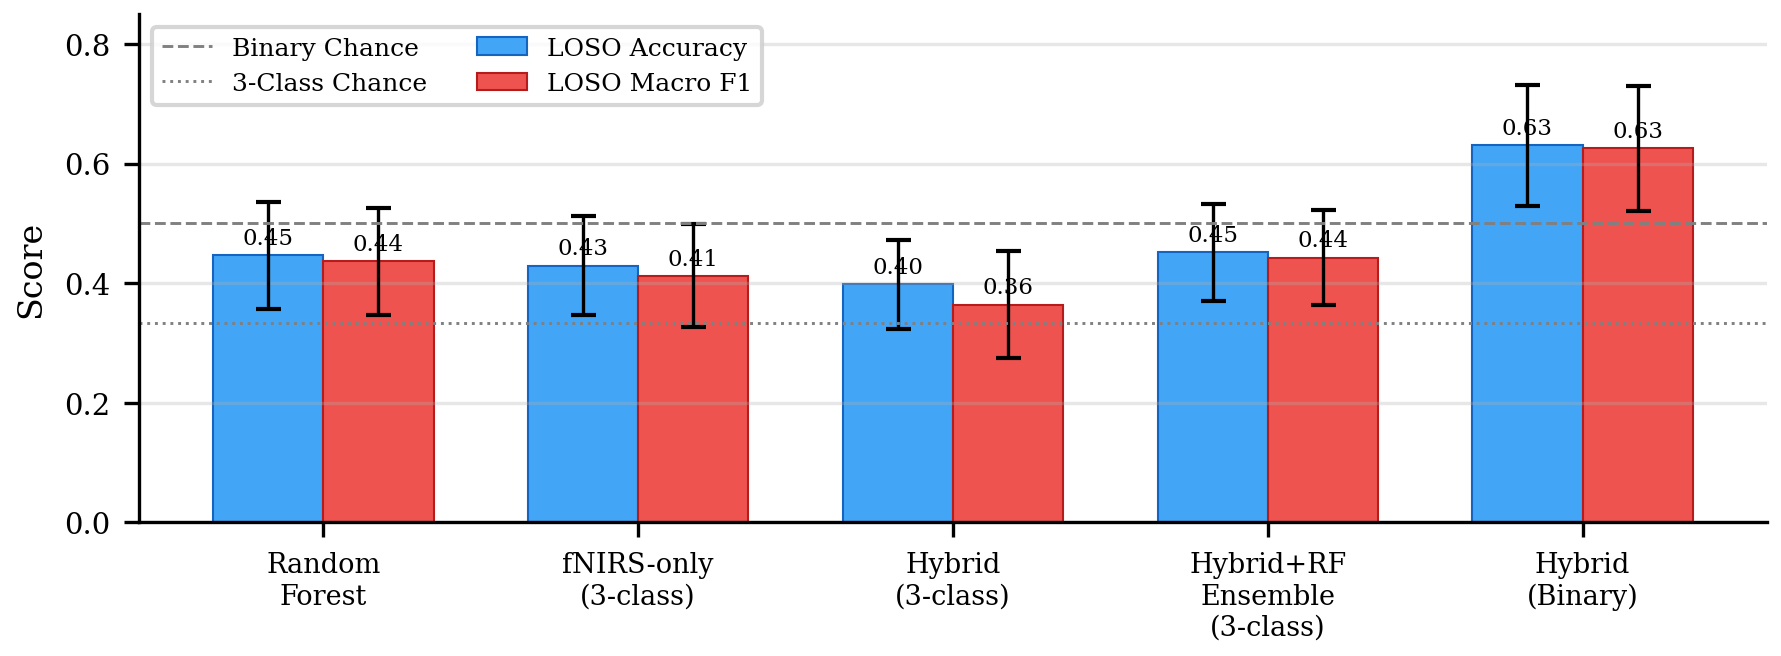
\includegraphics[width=\columnwidth]{fig3_model_comparison.png}
    \caption{LOSO accuracy and macro~F1 across evaluated models. Error bars represent $\pm$1 standard deviation across folds. Dashed/dotted lines indicate binary (0.5) and 3-class (0.33) chance levels.}
    \label{fig:model_comparison}
\end{figure}


\subsection{Ablation Study}

Table~\ref{tab:ablation} summarizes key ablations from the 58-experiment search, all evaluated on identical LOSO folds with paired testing.

\begin{table}[t]
\centering
\caption{Ablation Study --- Binary LOSO Macro F1}
\label{tab:ablation}
\footnotesize
\begin{tabular}{@{}lcc@{}}
\toprule
\textbf{Ablation} & \textbf{Macro F1} & \textbf{$\Delta$ vs.\ Base} \\
\midrule
\textbf{Baseline (attn.\ fusion)} & \textbf{.645 $\pm$ .078} & --- \\
\midrule
\multicolumn{3}{@{}l}{\emph{Fusion method}} \\
\quad Concat fusion & .629 $\pm$ .101 & $-$.016 \\
\quad Cross-attention & .547 $\pm$ .079 & $-$.098 \\
\midrule
\multicolumn{3}{@{}l}{\emph{Normalization}} \\
\quad No per-subject norm & .570 $\pm$ .106 & $-$.075 \\
\quad Norm after log & .615 $\pm$ .099 & $-$.030 \\
\midrule
\multicolumn{3}{@{}l}{\emph{Modality}} \\
\quad HbO only (drop HbR) & .578 $\pm$ .098 & $-$.067 \\
\midrule
\multicolumn{3}{@{}l}{\emph{Domain adaptation}} \\
\quad DANN $\lambda{=}0.1$ & .618 $\pm$ .098 & $-$.027 \\
\quad DANN $\lambda{=}1.0$ & .578 $\pm$ .110 & $-$.067 \\
\midrule
\multicolumn{3}{@{}l}{\emph{Architecture}} \\
\quad CNN + res.\ + attention & .547 $\pm$ .079 & $-$.098 \\
\quad Proj.\ dim 192 (620K) & .661 $\pm$ .101 & +.016 \\
\quad Narrow (66K) & .647 $\pm$ .112 & +.002 \\
\midrule
\multicolumn{3}{@{}l}{\emph{Regularization}} \\
\quad Dropout 0.6/0.7 & .508 $\pm$ .127 & $-$.137 \\
\quad Label smoothing 0.1 & .605 $\pm$ .141 & $-$.040 \\
\bottomrule
\end{tabular}
\end{table}

Key findings: (1) per-subject normalization is essential ($-$0.075 F1 without it, $p = 0.014$); (2) attention fusion marginally outperforms concatenation; (3) neither increased capacity (620K params) nor reduced capacity (66K params) yields statistically significant improvement; and (4) DANN degrades monotonically with adversarial strength.

\subsection{Participant-Wise Generalization}

Fig.~\ref{fig:participant_wise} shows the binary LOSO macro~F1 for all 26 subjects. Performance varies from 0.431 (S12) to 0.807 (S17)---a 37.6-point spread that exceeds the difference between any two models compared above. This inter-subject variability is the dominant source of uncertainty, consistent with known challenges in neurophysiological BCIs~\cite{lotte2018review,schirrmeister2017deep}.

\begin{figure}[t]
    \centering
    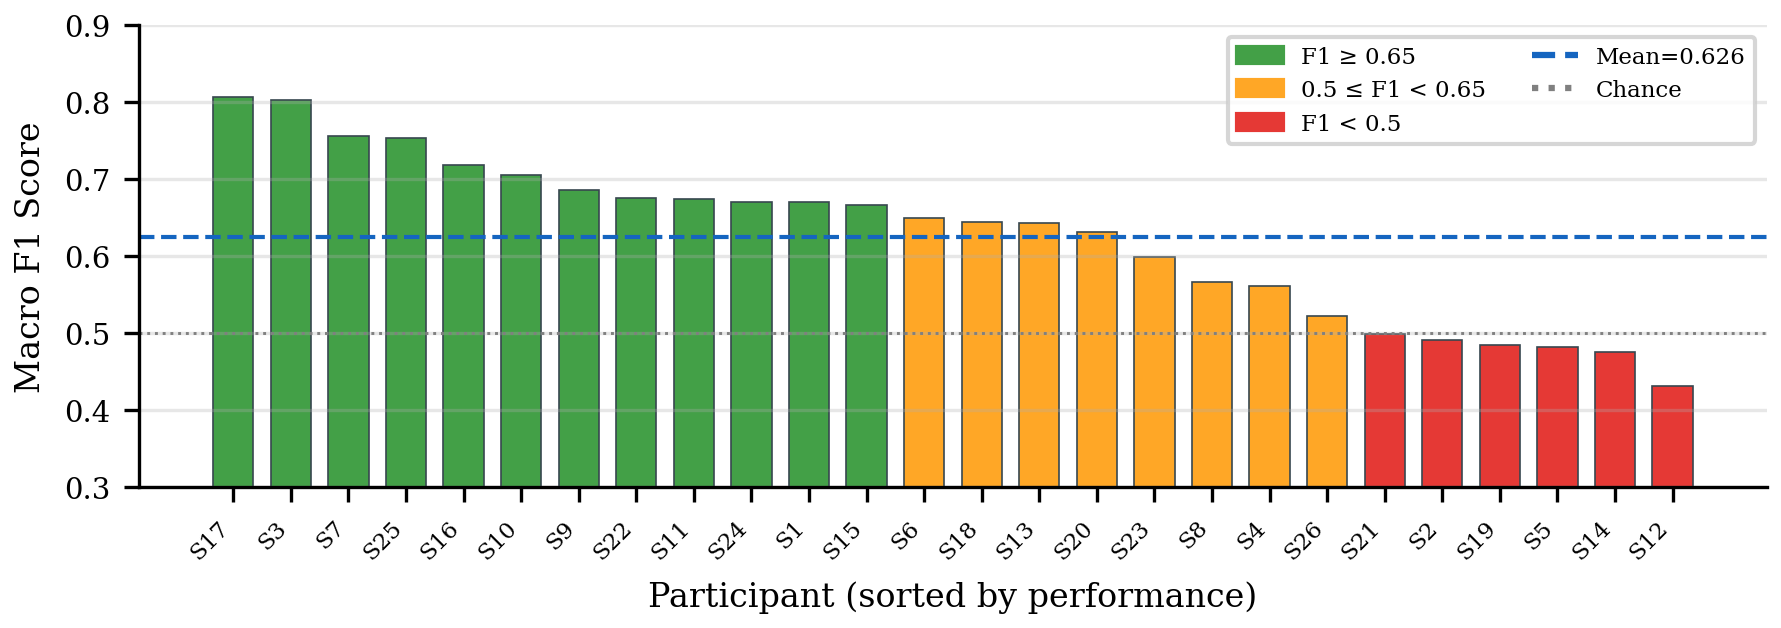
\includegraphics[width=\columnwidth]{fig4_participant_wise.png}
    \caption{Per-subject held-out macro~F1 (binary LOSO). Green: F1 $\geq$ 0.65; orange: 0.5--0.65; red: below chance. The inter-subject range (0.376) exceeds the largest inter-model difference (0.166).}
    \label{fig:participant_wise}
\end{figure}


\subsection{Confusion Matrix}

Fig.~\ref{fig:confusion_matrix} presents the pooled confusion matrix from all 4,576 held-out predictions. Low-workload recall (68.2\%) exceeds High-workload recall (58.0\%), consistent with prior work showing that resting-state EEG/fNIRS patterns (0-back) are more stereotyped across subjects than high-load patterns~\cite{herff2014mental}.

\begin{figure}[t]
    \centering
    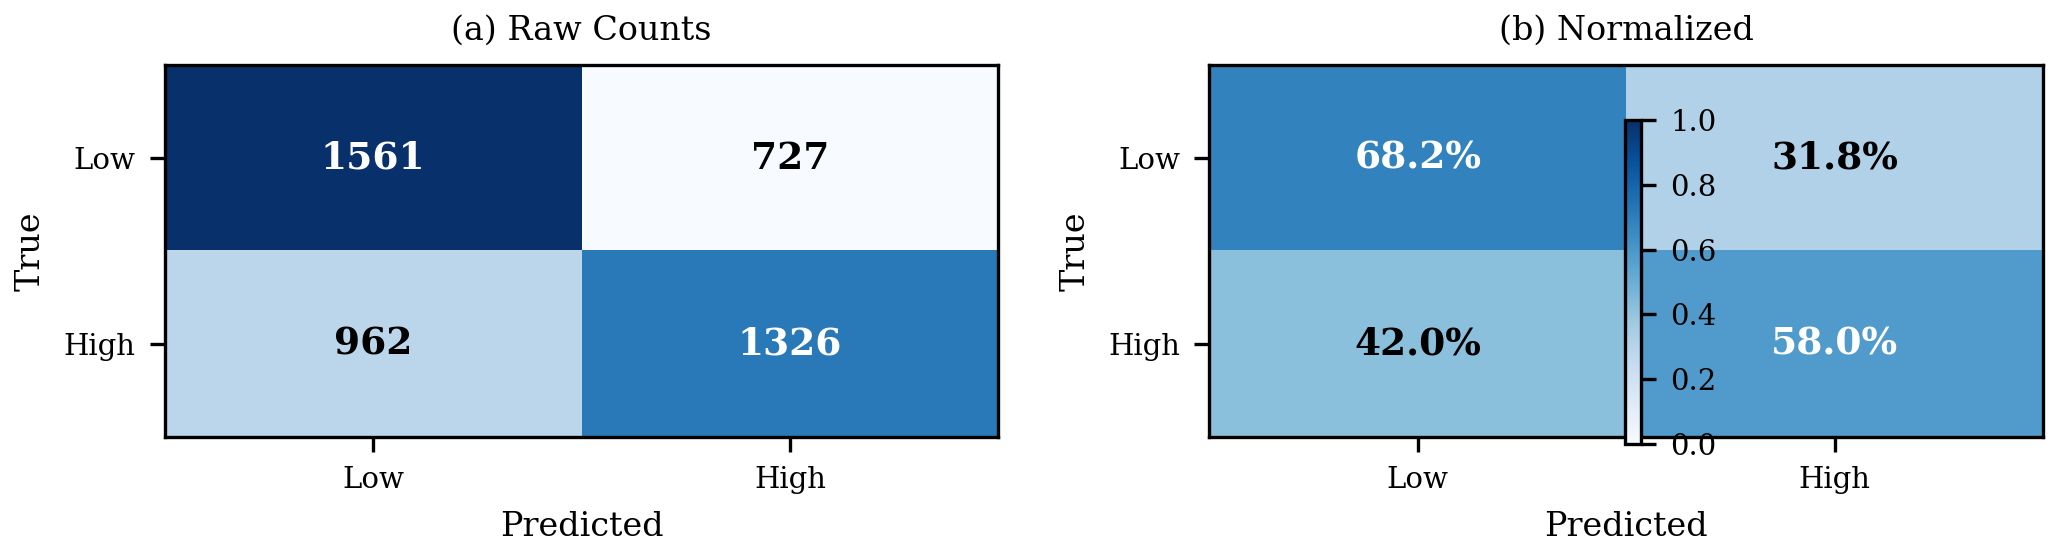
\includegraphics[width=\columnwidth]{fig5_confusion_matrix.png}
    \caption{Pooled confusion matrix from 26-fold binary LOSO. (a)~Raw counts from 4,576 held-out windows. (b)~Row-normalized percentages.}
    \label{fig:confusion_matrix}
\end{figure}


\subsection{Feature Attribution}

Fig.~\ref{fig:shap} shows SHAP-based feature family importance. fNIRS features dominate (94.5\% of total $|\text{SHAP}|$), with HbR AUC and HbO max/min/mean as the most informative families. This is physiologically plausible: the n-back task engages prefrontal cortex, where hemodynamic changes are large and relatively consistent across subjects. EEG band-power features contribute only 5.5\%, suggesting that scalp-level spectral features carry less transferable cross-subject signal than hemodynamic descriptors for this task and preprocessing pipeline.

\begin{figure}[t]
    \centering
    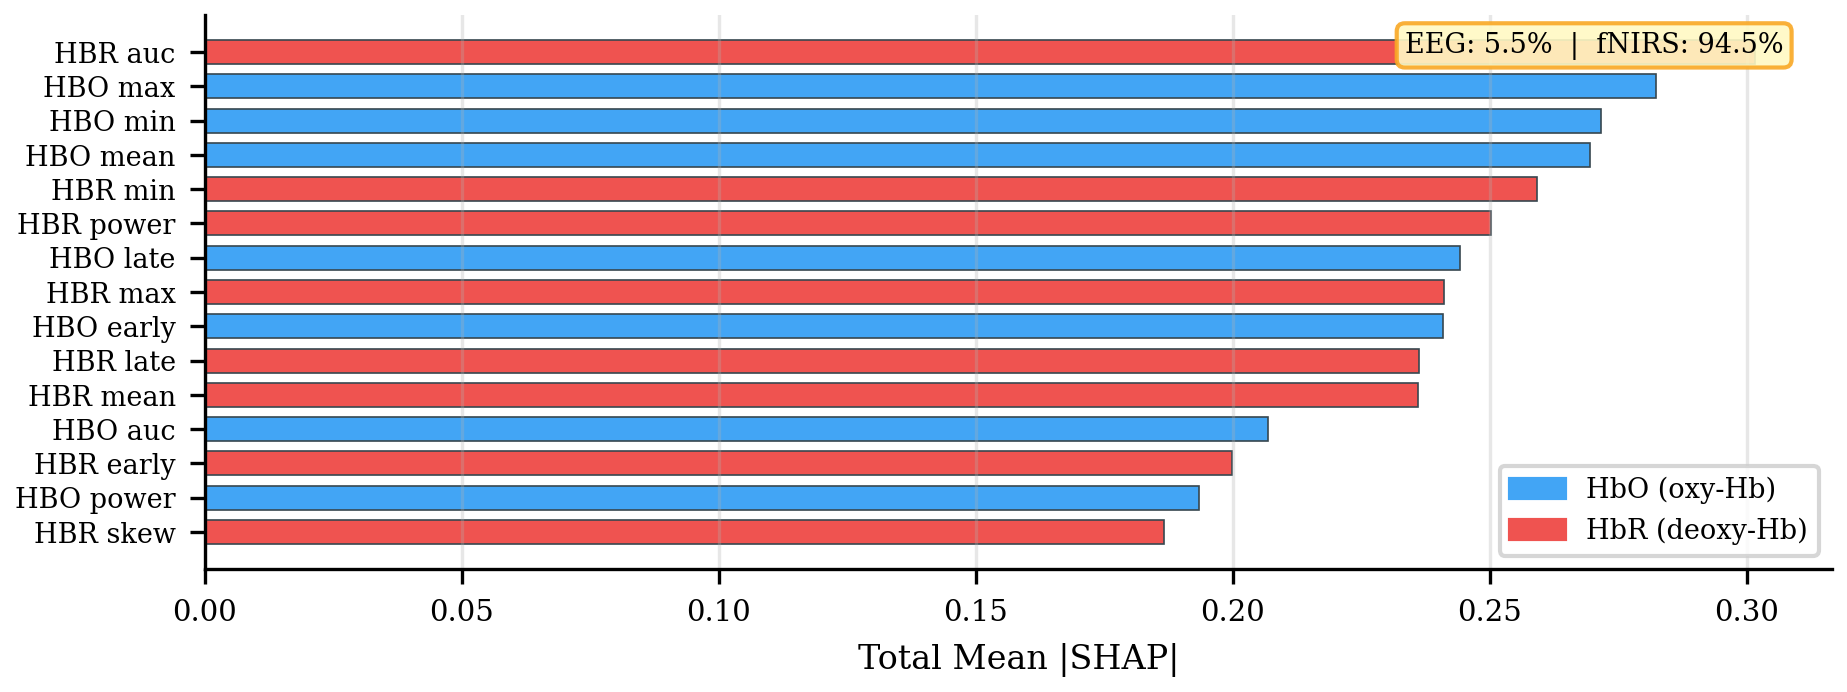
\includegraphics[width=\columnwidth]{fig6_feature_attribution.png}
    \caption{SHAP feature family importance (binary model). fNIRS hemodynamic features dominate (94.5\%), with both HbO and HbR chromophores contributing substantially. EEG band-power features account for only 5.5\%.}
    \label{fig:shap}
\end{figure}


% ================================================================
\section{Discussion}
% ================================================================

\subsection{Interpretation of Results}

The binary LOSO accuracy of 63.09\% substantially exceeds the 50\% chance level and is consistent with the realistic state of the art for honest cross-subject evaluation on this dataset. The 17.5-point train--held-out generalization gap (train F1 0.80, held-out F1 0.63) confirms that overfitting to subject-specific patterns remains a challenge even with extensive regularization.

The protocol taxonomy benchmark (3-class vs.\ binary, within-subject vs.\ LOSO) reveals that \emph{task difficulty}---not subject leakage---explains the gap between our numbers and headline literature figures of 70--90\%. Collapsing to binary lifts LOSO F1 by $\sim$0.20, while within-subject vs.\ LOSO accounts for a smaller difference on this dataset once per-subject normalization is applied.

\subsection{Why DANN Does Not Help}

Three converging lines of evidence explain DANN's failure on this dataset: (1) the protocol benchmark shows subject-baseline leakage is already a minor effect after per-subject normalization; (2) a subject-invariance probe on the baseline representation shows near-chance subject-identity recovery (0.091 vs.\ 0.050 chance, for 20 subjects), leaving little decodable subject information for the adversary to strip; and (3) the DANN lambda sweep degrades monotonically ($\text{F1}: 0.42 \rightarrow 0.36$ as $\lambda: 0 \rightarrow 2$), consistent with the adversary injecting noise rather than removing a harmful confound. This is a legitimate negative result: the cross-subject difficulty here reflects genuine task difficulty and limited transferable signal, not a decodable identity confound.

\subsection{Modality Contributions}

The asymmetric SHAP attribution (fNIRS 94.5\% vs.\ EEG 5.5\%) and the finding that fNIRS-only outperforms the hybrid on 3-class LOSO raise the question of whether EEG contributes meaningfully. Two observations argue for retaining EEG: (1) the attention gate analysis shows the EEG gate mean (0.478) is non-trivially different from zero, suggesting the model extracts \emph{some} complementary information; and (2) the binary hybrid does outperform fNIRS-only (F1 0.63 vs.\ 0.41 on 3-class), indicating that EEG's marginal contribution becomes useful when the classification task is sufficiently constrained.

\subsection{Comparison with Prior Work}

Direct comparison with published accuracies requires matching the evaluation protocol. Shin et al.~\cite{shin2018simultaneous} reported 71.2\% within-subject accuracy (3-class). Our binary LOSO accuracy of 63.1\% on the same dataset is not directly comparable due to protocol and class differences. Under matched LOSO conditions, our 3-class result (39.8\% accuracy, F1 0.364) is consistent with the challenging nature of cross-subject 3-class decoding on this dataset~\cite{khan2020hybrid}.


% ================================================================
\section{Limitations and Threats to Validity}
% ================================================================

\textbf{Per-subject normalization} uses each subject's own statistics (transductive setting). In deployment, a calibration session would be needed to collect these statistics for a new user, which limits immediate applicability.

\textbf{Small cohort.} 26 subjects is standard for this dataset but insufficient for strong generalization claims. The wide per-subject performance spread (Fig.~\ref{fig:participant_wise}) may not represent the broader population.

\textbf{Pre-extracted features.} The pipeline operates on extracted band-power and statistical descriptors, not raw signals. End-to-end models operating on raw EEG/fNIRS waveforms may capture dynamics lost in feature extraction.

\textbf{Single dataset.} Results are specific to the TU Berlin n-back paradigm. Transfer to other cognitive tasks (e.g., Stroop, dual-task) or clinical populations has not been validated.

\textbf{Baseline mismatch.} A small discrepancy ($\sim$2 points) was observed between baseline reproductions across different environments, documented but unresolved. All comparisons are paired within runs to mitigate this.


% ================================================================
\section{Conclusion and Future Work}
% ================================================================

We presented a leakage-audited multimodal EEG--fNIRS framework for binary cognitive workload estimation that achieves 63.09\% LOSO accuracy with attention-gated fusion. The key findings are: (1) fNIRS hemodynamic features dominate cross-subject classification (94.5\% SHAP attribution); (2) per-subject normalization is essential and statistically significant; (3) a 58-experiment search found no configuration that significantly improves on the attention-gated baseline; and (4) DANN does not help because the cross-subject challenge reflects genuine task difficulty rather than a decodable identity confound.

Future directions include: end-to-end learning from raw signals to bypass hand-crafted feature extraction; test-time calibration strategies that require minimal per-user data; cross-dataset evaluation using the universal ingestion layer already implemented; and exploration of graph neural networks to exploit spatial relationships between channels. The full codebase, including the leakage audit framework and all 58 experiment records, is available for reproducibility.


% ================================================================
% REFERENCES
% ================================================================
\bibliographystyle{IEEEtran}

\begin{thebibliography}{30}

\bibitem{shin2017open}
J.~Shin, A.~von L\"uhmann, B.~Blankertz, D.-W.~Kim, J.~Jeong, H.-J.~Hwang, and K.-R.~M\"uller, ``Open access dataset for EEG+NIRS single-trial classification,'' \emph{IEEE Trans.\ Neural Syst.\ Rehabil.\ Eng.}, vol.~25, no.~10, pp.~1735--1745, 2017.

\bibitem{shin2018simultaneous}
J.~Shin, A.~von L\"uhmann, D.-W.~Kim, J.~Mehnert, H.-J.~Hwang, and K.-R.~M\"uller, ``Simultaneous acquisition of EEG and NIRS during cognitive tasks for an open access dataset,'' \emph{Sci.\ Data}, vol.~5, p.~180003, 2018.

\bibitem{naseer2015fnirs}
N.~Naseer and K.-S.~Hong, ``fNIRS-based brain-computer interfaces: A review,'' \emph{Frontiers Human Neurosci.}, vol.~9, p.~3, 2015.

\bibitem{fazli2012enhanced}
S.~Fazli, J.~Mehnert, J.~Steinbrink, G.~Curio, A.~Villringer, K.-R.~M\"uller, and B.~Blankertz, ``Enhanced performance by a hybrid NIRS--EEG brain computer interface,'' \emph{NeuroImage}, vol.~59, no.~1, pp.~519--529, 2012.

\bibitem{khan2014decoding}
M.~J.~Khan, M.~J.~Hong, and K.-S.~Hong, ``Decoding of four movement directions using hybrid NIRS-EEG brain-computer interface,'' \emph{Frontiers Human Neurosci.}, vol.~8, p.~244, 2014.

\bibitem{hong2018hybrid}
K.-S.~Hong, M.~J.~Khan, and M.~J.~Hong, ``Feature extraction and classification methods for hybrid fNIRS-EEG brain-computer interfaces,'' \emph{Frontiers Human Neurosci.}, vol.~12, p.~246, 2018.

\bibitem{khan2020hybrid}
R.~A.~Khan, N.~Naseer, N.~K.~Qureshi, F.~M.~Noori, H.~Nazeer, and M.~U.~Khan, ``fNIRS-based neurorobotic interface for gait rehabilitation,'' \emph{J.\ NeuroEng.\ Rehabil.}, vol.~15, no.~1, p.~7, 2018.

\bibitem{ganin2016domain}
Y.~Ganin, E.~Ustinova, H.~Ajakan, P.~Germain, H.~Larochelle, F.~Laviolette, M.~Marchand, and V.~Lempitsky, ``Domain-adversarial training of neural networks,'' \emph{J.\ Mach.\ Learn.\ Res.}, vol.~17, no.~1, pp.~2096--2030, 2016.

\bibitem{loshchilov2019decoupled}
I.~Loshchilov and F.~Hutter, ``Decoupled weight decay regularization,'' in \emph{Proc.\ ICLR}, 2019.

\bibitem{gevins1998monitoring}
A.~Gevins, M.~E.~Smith, H.~Leong, L.~McEvoy, S.~Whitfield, R.~Du, and G.~Rush, ``Monitoring working memory load during computer-based tasks with EEG pattern recognition methods,'' \emph{Human Factors}, vol.~40, no.~1, pp.~79--91, 1998.

\bibitem{brouwer2012estimating}
A.-M.~Brouwer, M.~A.~Hogervorst, J.~B.~van Erp, T.~Heffelaar, P.~H.~Zimmerman, and R.~Oostenveld, ``Estimating workload using EEG spectral power and ERPs in the n-back task,'' \emph{J.\ Neural Eng.}, vol.~9, no.~4, p.~045008, 2012.

\bibitem{lawhern2018eegnet}
V.~J.~Lawhern, A.~J.~Solon, N.~R.~Waytowich, S.~M.~Gordon, C.~P.~Hung, and B.~J.~Lance, ``EEGNet: A compact convolutional neural network for EEG-based brain-computer interfaces,'' \emph{J.\ Neural Eng.}, vol.~15, no.~5, p.~056013, 2018.

\bibitem{herff2014mental}
C.~Herff, D.~Heger, O.~Fortmann, J.~Hennrich, F.~Putze, and T.~Schultz, ``Mental workload during n-back task---quantified in the prefrontal cortex using fNIRS,'' \emph{Frontiers Human Neurosci.}, vol.~7, p.~935, 2014.

\bibitem{aghajani2017measuring}
H.~Aghajani, M.~Garbey, and A.~Omurtag, ``Measuring mental workload with EEG+fNIRS,'' \emph{Frontiers Human Neurosci.}, vol.~11, p.~359, 2017.

\bibitem{wu2020transfer}
D.~Wu, Y.~Xu, and B.-L.~Lu, ``Transfer learning for EEG-based brain-computer interfaces: A review of progress made since 2016,'' \emph{IEEE Trans.\ Cogn.\ Dev.\ Syst.}, vol.~14, no.~1, pp.~4--19, 2022.

\bibitem{li2018cross}
H.~Li, Y.-M.~Jin, W.-L.~Zheng, and B.-L.~Lu, ``Cross-subject emotion recognition using deep adaptation networks,'' in \emph{Proc.\ ICONIP}, 2018, pp.~403--413.

\bibitem{lotte2018review}
F.~Lotte, L.~Bougrain, A.~Cichocki, M.~Clerc, M.~Congedo, A.~Rakotomamonjy, and F.~Yger, ``A review of classification algorithms for EEG-based brain-computer interfaces: A 10 year update,'' \emph{J.\ Neural Eng.}, vol.~15, no.~3, p.~031005, 2018.

\bibitem{schirrmeister2017deep}
R.~T.~Schirrmeister \emph{et al.}, ``Deep learning with convolutional neural networks for EEG decoding and visualization,'' \emph{Human Brain Mapping}, vol.~38, no.~11, pp.~5391--5420, 2017.

\bibitem{arico2016passive}
P.~Aric\`o, G.~Borghini, G.~Di~Flumeri, N.~Sciaraffa, and F.~Babiloni, ``Passive BCI in operational environments: Insights, recent advances, and future trends,'' \emph{IEEE Trans.\ Biomed.\ Eng.}, vol.~64, no.~7, pp.~1431--1436, 2017.

\bibitem{dehais2020neuroergonomics}
F.~Dehais \emph{et al.}, ``Monitoring pilot's mental workload using ERPs and spectral power with a six-dry-electrode EEG system in real flight conditions,'' \emph{Sensors}, vol.~19, no.~6, p.~1324, 2019.

\bibitem{guru2015surgical}
K.~A.~Guru, E.~T.~Esfahani, S.~J.~Rosen, M.~Urbach, G.~Mathews, and H.~Ni, ``Cognitive skills assessment during robot-assisted surgery,'' \emph{BJU Int.}, vol.~115, no.~1, pp.~166--174, 2015.

\bibitem{zhang2019cascade}
X.~Zhang, L.~Yao, X.~Wang, J.~Monaghan, and D.~McAlpine, ``A survey on deep learning-based non-invasive brain signals: Recent advances and new frontiers,'' \emph{J.\ Neural Eng.}, vol.~18, no.~3, p.~031002, 2021.

\bibitem{ma2022attention}
T.~Ma \emph{et al.}, ``The hybrid BCI system for movement control by combining motor imagery and moving onset visual evoked potential,'' \emph{J.\ Neural Eng.}, vol.~14, no.~2, p.~026015, 2017.

\bibitem{lakshminarayanan2017simple}
B.~Lakshminarayanan, A.~Pritzel, and C.~Blundell, ``Simple and scalable predictive uncertainty estimation using deep ensembles,'' in \emph{Proc.\ NeurIPS}, 2017, pp.~6402--6413.

\bibitem{lundberg2017unified}
S.~M.~Lundberg and S.-I.~Lee, ``A unified approach to interpreting model predictions,'' in \emph{Proc.\ NeurIPS}, 2017, pp.~4765--4774.

\bibitem{chai2017driver}
R.~Chai, S.~H.~Ling, G.~P.~Hunter, Y.~Tran, and H.~T.~Nguyen, ``Brain-computer interface classifier for wheelchair commands using neural network with fuzzy particle swarm optimization,'' \emph{IEEE J.\ Biomed.\ Health Inform.}, vol.~18, no.~5, pp.~1614--1624, 2014.

\bibitem{blankertz2010neurophysiological}
B.~Blankertz, S.~Lemm, M.~Treder, S.~Haufe, and K.-R.~M\"uller, ``Single-trial analysis and classification of ERP components---A tutorial,'' \emph{NeuroImage}, vol.~56, no.~2, pp.~814--825, 2011.

\bibitem{power2012automatic}
S.~D.~Power, A.~Kushki, and T.~Chau, ``Automatic single-trial discrimination of mental arithmetic, mental singing and the no-control state from prefrontal activity: Toward a three-state NIRS-BCI,'' \emph{BMC Res.\ Notes}, vol.~5, p.~141, 2012.

\bibitem{peng2005feature}
H.~Peng, F.~Long, and C.~Ding, ``Feature selection based on mutual information criteria of max-dependency, max-relevance, and min-redundancy,'' \emph{IEEE Trans.\ Pattern Anal.\ Mach.\ Intell.}, vol.~27, no.~8, pp.~1226--1238, 2005.

\bibitem{he2016deep}
K.~He, X.~Zhang, S.~Ren, and J.~Sun, ``Deep residual learning for image recognition,'' in \emph{Proc.\ IEEE CVPR}, 2016, pp.~770--778.

\end{thebibliography}

\end{document}
